%%%%%%%%%%%%%%%%%%%%%%%%%%%%%%%%%%%%%%%%%%%%%%%%%%%%%%%%%%%%%%%%%%%%%%%%%%%%%%%%

% IEEEconf.cls file must exist in the same directory as the TeX file you want to compile
\documentclass[letterpaper, 10 pt, conference]{IEEEconf}

\title{\LARGE \bf
COMPUTER HISTORY\\
\large Hard Drives, Storage Mediums, and RAM
}

\author{git-group 2\\
\small Aidan Clevenger\\
\small John Runyon\\
\small Benjamin Salazar\\
}

% Image/graphics support
\usepackage{graphicx}
\graphicspath{ {./images/} }

% Formatting for lists
\usepackage{enumitem}

% Formatting for media
\usepackage{float}
\restylefloat{table}
\restylefloat{figure}

\begin{document}


\maketitle
\thispagestyle{empty}
\pagestyle{empty}


%%%%%%%%%%%%%%%%%%%%%%%%%%%%%%%%%%%%%%%%%%%%%%%%%%%%%%%%%%%%%%%%%%%%%%%%%%%%%%%%
\section*{ABSTRACT}
\textit{
Today we are used to having many different easy ways of transferring data on drives. Well, It wasn't always as simple. In this paper we will be discussing how HDD's (hard drives) got their start, as well as RAM, (Random Access Memory) which is critical to our computers today.
}

%%%%%%%%%%%%%%%%%%%%%%%%%%%%%%%%%%%%%%%%%%%%%%%%%%%%%%%%%%%%%%%%%%%%%%%%%%%%%%%%
\section{INTRODUCTION}

The topic we chose was "Memory and Storage," and we chose this topic because it is something we all need and hold as important, but very few of us really think about storage very often. Before HDD's - paper or other writing implements were used, paintings were painted and that was about it. Storage of important data was out of sight and an impossibility. Now, anyone anywhere can store their valuable photos or documents with ease. 

RAM is an important (That might be an understatement, because without RAM your device would never turn on) part of your device. It holds your tabs and other files held in the background.

%%%%%%%%%%%%%%%%%%%%%%%%%%%%%%%%%%%%%%%%%%%%%%%%%%%%%%%%%%%%%%%%%%%%%%%%%%%%%%%%
\section{TIME PERIOD}
Different forms of information storage have been in use for centuries.These forms include Human memory, art, and writing. However, it was only very recently that humanity created a way to create and store digital information. This digital storage device was the vacuum tube and it was first invented in 1904 by John Ambrose Fleming. Later in 1951 the vacuum tube was used in the first computer as an information storage device. Then in 1953 vacuum tubes were switched out for magnetic core memory. Magnetic core memory was first invented in 1948 by An Wang and was used some in 1950. However it really did not gain prevalence until 1953. Magnetic core memory was the standard from 1953 all the way until the 1970's when early RAM became the standard. Invented in 1968 by Robert Heath Dennard, RAM became the standard for digital information storage and is still used today in modern computers. 

%%%%%%%%%%%%%%%%%%%%%%%%%%%%%%%%%%%%%%%%%%%%%%%%%%%%%%%%%%%%%%%%%%%%%%%%%%%%%%%%

\begin{figure}[h!]
\centering
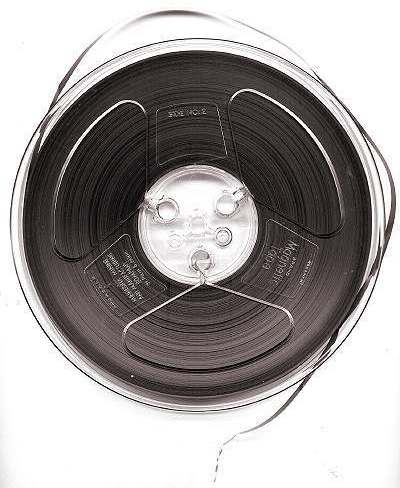
\includegraphics[width=0.3\textwidth]{Magtape1.jpg}
\caption{Early Magnetic Tape}
\label{fig:example}
\end{figure} 

\section{COMPUTER HARDWARE}
Magnetic tapes, disks, and Semiconductors are all used to store digital information. Magnetic tapes were primarily used to store audio recordings.The magnetic tape drives store data by arranging it into long strands that run the length of the tape. Disks are used to store any kind of digital information. Information is stored on the disks in binary. Semiconductors use RAM to store information. They do this by either going back and forth from one to zero and accessing bits directly or by holding a charge. A charged semiconductor stands for one while an uncharged stands for zero. This first case where the semiconductors access bits directly is known as SRAM. This latter method where semiconductors hold charge is known as DRAM. Disks and Semiconductors are used today. 

\section{COMPUTER SOFTWARE}

\section{CONCLUSION}
In conclusion, memory and storage ends up being one of if not the most important parts to modern computing, having roles to play in nearly every operation in a computer. Despite their many forms, they all manage to be useful in their own ways. From vacuum tubes to hard disks, all forms of storage are the foundation on which the modern world is built. Memory is often overshadowed by other parts that go into computers, processors often take the spotlight. However, searching for information on the subject has led us to find that memory is undoubtedly a crucial part to the computing world around us.


\section*{REFERENCES}

\begin{enumerate}[label={[\arabic*]}]

\item Computer History Museum, Revolution [Online]. 
\item Wikipedia, Computer Memory [Online]
\item Wikipedia, Magnetic Tape [Online]
\end{enumerate}

\end{document}

